\chapter*{Introduction}
	Dans le cadre du module de \emph{Réseaux}, le projet de travaux pratiques portait sur la réalisation d'un protocole ou d'une application d'échange de données. Dans ce rapport, nous allons présenter les logiciels qui forment notre suite de messagerie instantanée que nous avons réalisé et qui permet l'échange de texte entre plusieurs clients via un serveur central. Ces programmes ont été réalisés dans le langage C comme précisé dans le sujet et utilisent les sockets bas niveau.
	
	Dans ce rapport, nous allons présenter dans un premier temps notre analyse du sujet et la manière dont nous avons pensé notre application. Ensuite, nous présenterons le fonctionnement de l'application en examinant les logiciels côté serveur puis client. 
		
\chapter{Analyse}
	\section{Présentation du sujet}
		Le sujet de ce projet portait sur la réalisation de programmes communiquants via le réseau via une architecture client / serveur.  Pour cela, nous devions utiliser le langage C, un des plus utilisé au monde et dont la caractéristique principale est d'être bas niveau, ce qui permet d'être un bon outil d'enseignement. En effet, cela permet de voir les briques de base d'un logiciel sans être pollué par une surcouche haut niveau.
		
		Pour nous aider, nous avons bénéficié d'un exemple étudié en TP et qui montrait les fonctions principales d'envoi et de reception de messages, ainsi que la manière d'utiliser les threads pour paralléliser les tâches d'un programme. Cela permet de pouvoir écouter et émettre en continu pour chaque connexion établie.

	\section{Choix du projet}
		

	\section{Présentation des fonctionnalités}
		- salon général
		- messages privés
		

\chapter{Fonctionnement du Chat}
	
	\section{Présentation du protocole}
		Parce qu'un schéma est plus parlant qu'un long discours, commençons par une présentation du protocole sous la forme d'un diagramme de séquence. Il est important de rappeler que comme toute architecture client/serveur, le client envoie des requêtes (ici sous la forme de messages) au serveur qui lui s'occupe d'agit en conséquence.
		\begin{figure}[h!]
			\centering
			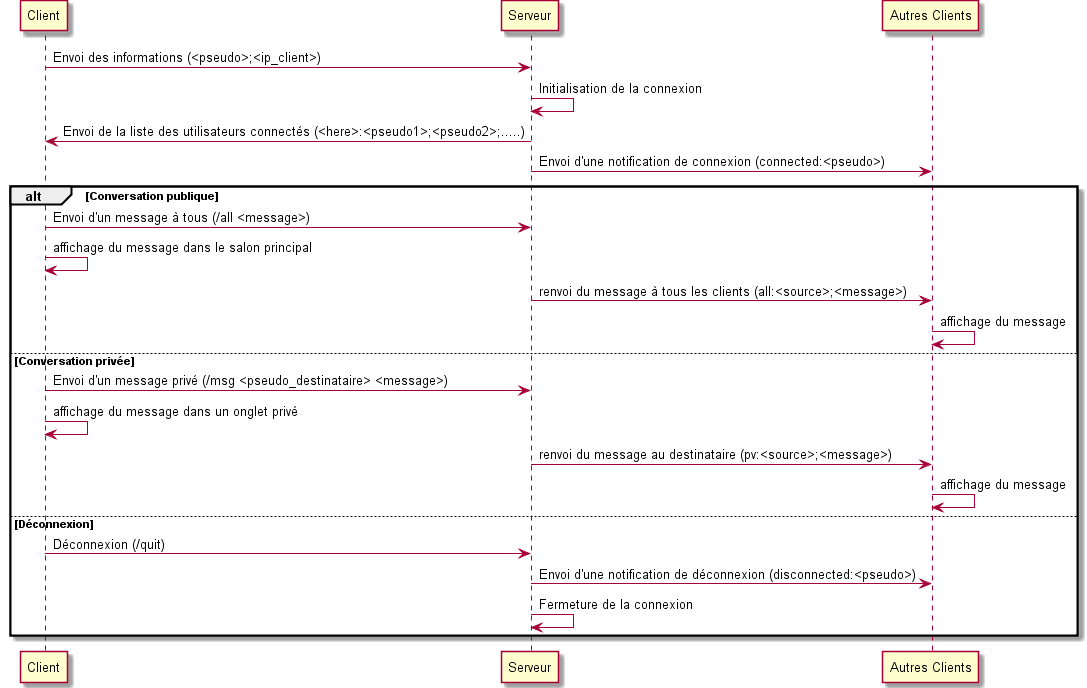
\includegraphics[scale=0.45]{protocol.png}
			\caption{Présentation générale du protocole utilisé}
		\end{figure}
		\FloatBarrier
		
		L'entité \emph{Client} représente le client à partir duquel nous présentons notre protocole. C'est cette entité qui envoie les requêtes au serveur. Étant donné que le serveur est un intermédiaire entre plusieurs clients, nous avions besoin d'une autre entité. L'entité \emph{Autres Clients} représente donc les autres clients connectés au serveur, clients que nous n'étudions pas (un seul suffit à comprendre les spécifications du protocole) mais qui nous sert ici à montrer à quels moments les messages envoyés par \emph{Client} sont retransmis.\\
		
		Nous remarquons ici qu'une fois la connexion initialisée (le client et le serveur se connaissent et le serveur est prêt à écouter), le client n'a que trois possibilités :
		\begin{itemize}
			\item Engager une conversation dans le salon général ;
			\item Engager une conversation privée ;
			\item Se déconnecter.
		\end{itemize}
		
		Le protocole est donc très simple. Mais l'implémentation l'est moins du fait que le serveur doive pouvoir gérer plusieurs clients simultannément. Nous détaillerons donc le fonctionnement du serveur dans le chapitre suivant.
		
	
	\section{Fonctionnement du serveur}
		
		Côté serveur, il nous a paru évident qu'il faille implémenter une file de messages à envoyer. Pour utiliser cette file correctement, nous avons donc besoin de deux threads par client : un thread qui scrute la réception des requêtes du client et qui agit en conséquence, ainsi qu'un thread qui parcourt constamment la file de message afin de récupérer les messages à envoyer au client pour les retransmettre ensuite.
	
		\subsection{Liste des utilisateurs connectés}
			détails de l'implémentation + quand est-ce qu'elle est mise à jour ?
			
		\subsection{File de messages}
			idem\\
			ne pas oublier de préciser la méthode de "pop"\\
			ne pas oublier de parler du mutex
			
		\subsection{Thread de lecture}
			se présente sous la forme d'un protocole (1 string = 1 action)
			
		\subsection{Thread d'écriture}
			idem
			
	
	\section{Fonctionnement du client}
		\subsection{Le coeur de l'application}
	
	
		\subsection{L'interface graphique}
			

\chapter*{Conclusion}
	Ce projet aura été l'occasion de consolider nos connaissances dans le domaine du réseau, et plus particulièrement dans le domaine des applications client/serveur. En effet, nous avons mis en place une architecture permettant à de multiples clients de partager des données (et plus particulièrement du texte) en passant par un serveur centralisé. Cela nous a permis de manipuler des sockets et des threads, éléments essentiels à tout informaticien lorsqu'il s'agit de faire des logiciels modernes : ils permettent l'interaction avec le réseau et la parallélisation des tâches.
	
	Parmi les évolutions envisageables, il sera possible dans une prochaine version de notre logiciel de s'affranchir du serveur centralisé pour réaliser une application répartie. Cela permettra de discuter sans dépendre d'une entité principale qui peut être surchargée ou indisponible, chaque client faisant aussi office de serveur. Notons aussi qu'il est possible de faire transiter par le réseau des fichiers pour permettre l'envoi de pièces jointes d'une machine à l'autre. Cette partie a été envisagée pendant le développement mais nous avons finalement décidé de nous concentrer sur les tâches les plus prioritaires et sur la correction de bogues.
